\documentclass[11pt]{article}

\usepackage[spanish]{babel}
\usepackage[margin=1in]{geometry}
\usepackage{amsmath, amssymb, amsfonts}
\usepackage{graphicx}
\usepackage{booktabs}
\usepackage{array}
\usepackage{enumitem}
\usepackage{tcolorbox}
\usepackage{hyperref}
\usepackage{xcolor}
\usepackage{float}
\usepackage{csquotes}
\usepackage{parskip}
\usepackage{pgfplots}
\usepackage[backend=biber,style=numeric,sorting=none]{biblatex}
\addbibresource{referencias.bib}

\usetikzlibrary{arrows.meta, positioning}
\pgfplotsset{compat=1.18}

\setlist{itemsep=2pt, topsep=4pt}

\title{\textbf{Proyecto 2: Detección de Lavado de Dinero} \vspace{1em}\\
  Deep Learning y Sistemas Inteligentes - CC3092}
\author{José Antonio Mérida Castejón}
\date{\today}

\begin{document}
\decimalpoint

\maketitle

\section*{Resumen ejecutivo}

\textbf{Sistema.} El proyecto construye un sistema que ordena a los remitentes de una remesadora según qué tan probable es que estén lavando dinero. Cada alerta indica las transacciones que la provocaron. El sistema tiene dos etapas. La Etapa A aprende cómo se ve el comportamiento normal, sin usar etiquetas de lavado. La Etapa B aprende de casos ya etiquetados a reconocer el lavado, y parte de lo que aprendió la Etapa A.

\textbf{Datos.} Se usó IBM AML (HI-Small), un conjunto sintético de cinco millones de transacciones donde solo una de cada mil es lavado. No hay datos reales etiquetados de remesas, por lo que las cifras describen un simulador y no una remesadora real.

\textbf{Resultados.}
\begin{itemize}
  \item Si el equipo revisa el 5\% de los remitentes con mayor riesgo, encuentra \textbf{78\% de los lavadores}.
  \item De esas alertas, \textbf{15\% son reales}. Los sistemas por reglas rondan entre 1\% y 5\%. El resto son falsos positivos, es decir, remitentes legítimos señalados por error. El sistema reduce la carga de revisión, pero no la elimina.
  \item El sistema de dos etapas \textbf{no supera} a un clasificador entrenado desde cero, sin la Etapa A. Solo lo iguala. Este es el resultado negativo del proyecto.
  \item La explicación de las alertas es útil. En dos de cada tres casos detectados, la transacción que el modelo más destaca es de lavado. Al azar, ocurriría menos de una vez de cada cuatro.
\end{itemize}

\textbf{Pendiente.} Hacen falta datos reales etiquetados, probabilidades calibradas y más corridas de entrenamiento (sección~\ref{sec:limites}).

\section{El problema de negocio y su contexto regulatorio}

Guatemala recibe más de USD 20 mil millones al año en remesas, cerca del 19\% del PIB. El corredor hacia Estados Unidos es de los más grandes del mundo. Son millones de pagos pequeños, y entre ellos es fácil esconder dinero ilícito. Una forma común es partir un monto grande en varios pagos chicos.

Por eso, las remesadoras y los bancos que reciben remesas deben detectar operaciones sospechosas y reportarlas. En Guatemala, la ley vigente es el Decreto 15-2026 \cite{decreto152026}, en vigor desde el 17 de septiembre de 2026. Esta ley reemplaza a los Decretos 67-2001 y 58-2005. El enunciado de este proyecto todavía cita el 67-2001, que ya no rige. El decreto exige evaluar el riesgo de cada cliente, monitorear sus operaciones y reportar las sospechosas a la Intendencia de Verificación Especial (IVE), que depende de la Superintendencia de Bancos. El reglamento con los detalles estaba pendiente al redactar este reporte.

A nivel internacional, el GAFI pide regular las transferencias de dinero y reportar transacciones sospechosas \cite{fatf2012}. En Estados Unidos, las remesadoras reportan actividad sospechosa ante FinCEN desde USD 2,000 \cite{fincen1022}.

El problema está en cómo se detecta hoy. Los sistemas basados en reglas alertan, por ejemplo, ante cualquier pago sobre cierto monto. Según el enunciado, entre 95\% y 99\% de esas alertas son falsos positivos. El equipo revisa cientos de alertas para encontrar un caso real, y los patrones más sofisticados pasan sin ser vistos. Además, una alerta sin explicación no sirve ante un regulador. El analista necesita saber qué transacciones la provocaron antes de abrir una investigación.

Este proyecto propone un sistema que ordena a los remitentes por nivel de riesgo y señala las transacciones responsables de cada alerta. El equipo revisa desde el más riesgoso hacia abajo, hasta donde alcance su capacidad.

\section{Datos y construcción de secuencias}

Se usó IBM AML (HI-Small) \cite{altman2023}, y no PaySim, porque simula bancos, personas y empresas con lavado inyectado en patrones conocidos. Además, sus remitentes tienen historia repetida, que es lo que necesita un modelo de secuencias. Se usó la variante HI-Small completa, sin submuestreo adicional. Es suficiente para entrenar, con más de cinco millones de transacciones y cerca de 497 mil remitentes, de los cuales 3,376 lavan en algún momento.

Antes de modelar, el análisis exploratorio dejó cuatro hallazgos que se volvieron decisiones.
\begin{itemize}
  \item \textbf{Las fechas no son confiables.} La actividad normal se detiene después del 10 de septiembre, pero el simulador sigue generando lavado. Por eso el modelo solo ve el tiempo transcurrido desde la transacción anterior del mismo remitente, sin fecha ni hora.
  \item \textbf{Un formato de pago concentra el lavado.} El formato ACH reúne el 87\% de las transacciones de lavado. Wire y Reinvestment no tienen ninguna. Estos remitentes se submuestrean en entrenamiento, es decir, se usa solo una parte de ellos, porque son casos seguros que enseñan una regla fácil.
  \item \textbf{El monto no basta para separar las clases.} Los montos de lavado suelen ser mayores, pero se traslapan mucho con los normales. Además, varían entre cantidades muy pequeñas y muy grandes. Por eso se usa el logaritmo del monto y su valor relativo a lo habitual del remitente.
  \item \textbf{Hay ocho patrones de lavado conocidos.} Se llaman tipologías. Por ejemplo, fan-in es cuando muchos remitentes pagan a un mismo receptor. Solo el 62\% de las transacciones de lavado pertenece a una tipología. No se usan para entrenar, porque serían etiquetas disfrazadas, y sirven para evaluar y explicar.
\end{itemize}

Cada remitente se representa con ventanas, que son tramos de hasta 32 transacciones seguidas, ordenadas en el tiempo. Una ventana es positiva si contiene al menos una transacción de lavado. La siguiente tabla resume las decisiones y su justificación.

\begin{table}[H]
\centering
\small
\begin{tabular}{>{\raggedright\arraybackslash}p{3cm}>{\raggedright\arraybackslash}p{5.4cm}>{\raggedright\arraybackslash}p{6.6cm}}
\toprule
Decisión & Elección & Justificación \\
\midrule
Variables de cada transacción & Monto (en logaritmo y relativo al remitente), tiempo desde la transacción anterior, receptor nuevo o conocido, remitentes que ya pagaron a ese receptor, formato y moneda de pago, y algunas banderas & Todas se calculan respecto al remitente y ninguna usa fecha ni hora. El número de remitentes del receptor da contexto de red y se calcula sin mirar el futuro \\
Normalización & Logaritmo del monto en USD y estandarización con datos de entrenamiento & Los montos varían mucho. Usar solo datos de entrenamiento evita filtrar información \\
Largo mínimo & 2 transacciones & Una sola no forma una secuencia. Bajar el mínimo de 3 a 2 recupera cerca de 500 remitentes positivos. Los de una sola transacción quedan fuera \\
Largo máximo & Ventanas de 32 transacciones, con avance de 16 y máximo de 12 por remitente & Cubre la historia de casi todos los remitentes. El solape evita cortar un patrón por el borde, y el tope evita que una cuenta muy activa domine \\
Desbalance & Submuestreo de Wire y Reinvestment. En la Etapa B, 40 negativos por positivo y una pérdida que da más peso a los casos raros & Solo 0.93\% de las ventanas de entrenamiento son positivas. Validación y prueba conservan la distribución real \\
División & 70\% entrenamiento, 15\% validación y 15\% prueba, por remitente & Las ventanas de un mismo remitente comparten transacciones. Separarlas entre conjuntos filtraría información \\
\bottomrule
\end{tabular}
\caption{Decisiones de datos y su justificación.}
\end{table}

La Etapa B entrena con cerca de 209 mil remitentes, de los cuales 2,270 son positivos. Validación y prueba tienen cerca de 51,600 remitentes cada uno, y la prueba incluye 486 positivos. El notebook comprueba que ningún remitente aparezca en dos conjuntos, y muestra ejemplos de secuencias normales y sospechosas. Las sospechosas no se distinguen a simple vista, porque tienen un solo pago de lavado entre transacciones de aspecto normal. La señal aparece al combinar monto, tiempo, receptor y formato, y por eso se usa un modelo de secuencias.

\section{Diseño del sistema}

\begin{figure}[ht]
\centering
\begin{tikzpicture}[
  node distance=7mm and 8mm,
  box/.style={draw, rounded corners=2pt, minimum height=8mm, align=center, font=\small, fill=gray!8},
  outbox/.style={draw, rounded corners=2pt, minimum height=8mm, align=center, font=\small, fill=blue!10},
  arr/.style={-{Stealth[length=2mm]}, thick}
]
\node[box] (a1) {Ventana de\\32 transacciones};
\node[box, right=of a1] (a2) {Encoder};
\node[box, right=of a2] (a3) {$z$\\(32 números)};
\node[box, right=of a3] (a4) {Decoder};
\node[outbox, right=of a4] (a5) {Error de\\reconstrucción};
\draw[arr] (a1)--(a2); \draw[arr] (a2)--(a3); \draw[arr] (a3)--(a4); \draw[arr] (a4)--(a5);
\node[left=2mm of a1, font=\bfseries\small, xshift=-2mm] {A};

\node[box, below=14mm of a1] (b1) {Ventana de\\32 transacciones};
\node[box, right=of b1] (b2) {Encoder\\(de la Etapa A\\o aleatorio)};
\node[box, right=of b2] (b3) {Attention\\pooling};
\node[box, right=of b3] (b4) {MLP};
\node[outbox, right=of b4] (b5) {P(lavado)\\+ heatmap};
\draw[arr] (b1)--(b2); \draw[arr] (b2)--(b3); \draw[arr] (b3)--(b4); \draw[arr] (b4)--(b5);
\node[left=2mm of b1, font=\bfseries\small, xshift=-2mm] {B};
\end{tikzpicture}
\caption{Las dos etapas. La Etapa A se entrena solo con remitentes normales y no usa etiquetas; la Etapa B usa etiquetas y puede partir del encoder de la Etapa A.}
\end{figure}

\subsection{Etapa A: aprender lo normal}

\textbf{Idea.} Hay muy pocos casos de lavado y el lavado cambia de forma. Por eso, en lugar de definir qué es sospechoso, el sistema aprende qué es normal, que es lo más abundante. Para esto se usa un autoencoder (Lab-03), una red neuronal con dos partes. El encoder resume cada ventana en 32 números, y el decoder intenta reconstruir la ventana a partir de ese resumen. Una ventana parecida a lo normal se reconstruye bien. Una ventana rara se reconstruye mal, y ese error de reconstrucción es el puntaje de anomalía. El decoder nunca ve la ventana original, porque si la viera podría copiarla completa, incluidas las anomalías. La Etapa A se entrena solo con remitentes que nunca lavaron.

\textbf{Arquitecturas comparadas.} Se compararon tres tipos de encoder, con la misma pérdida y el mismo entrenamiento, para que la única diferencia fuera la arquitectura. El primero es un MLP, una red simple que recibe la ventana completa sin considerar el orden. El segundo es un LSTM \cite{hochreiter1997}, una red que lee las transacciones una por una y mantiene una memoria de lo anterior (Lab-02). El tercero es un Transformer \cite{vaswani2017}, que usa un mecanismo de atención para que cada transacción pueda mirar a todas las demás de la ventana (Lab-04, Proyecto 1). Este tipo de red también se usa para detectar anomalías en series de tiempo \cite{xu2022}. Ambos terminan en una capa de attention pooling, que da un peso a cada transacción según su importancia. Esos pesos se usan después como mapa de calor.

\textbf{Puntaje y umbral.} El error de reconstrucción crece con el largo de la ventana. Un puntaje sin ajustar favorecería a los remitentes con más actividad. Por eso se compararon varias formas de calcularlo, y validación eligió la que promedia el error de las tres peores transacciones y lo normaliza por el largo de la ventana. El umbral de alerta es el puntaje que deja alertado al 5\% de los remitentes en validación, que representa la capacidad de revisión del equipo. Se descartó el umbral que maximiza el F1, una métrica que combina precisión y recall, porque alertaba a menos del 1\% de los remitentes.

\subsection{Etapa B: clasificador y transfer learning}
\label{sec:etapab}

La Etapa B es un clasificador. Recibe una ventana y calcula la probabilidad de que contenga lavado. Usa un encoder, una capa de attention pooling nueva y una red pequeña que entrega la probabilidad. La probabilidad de un remitente es la de su ventana más sospechosa. Un promedio diluiría una ventana mala entre muchas normales.

\textbf{Transfer learning (Semana 9, Lab-06).} Transfer learning consiste en reutilizar lo que una red aprendió en una tarea para resolver otra. Aquí hay solo 2,270 remitentes positivos de entrenamiento contra más de 200 mil normales. El encoder de la Etapa A ya vio a los normales, así que la hipótesis es que su representación ayuda al clasificador. Se probó con LSTM y con Transformer, para ver si la conclusión depende de la arquitectura. El MLP no se usa aquí porque no produce una representación por transacción. Cada arquitectura se entrenó de tres formas.
\begin{itemize}
  \item \textbf{Desde cero.} El encoder empieza con pesos aleatorios y aprende solo con etiquetas. Es la línea base. Si el sistema de dos etapas no la supera, la Etapa A no aporta.
  \item \textbf{Congelado.} Se usa el encoder de la Etapa A sin modificarlo, y solo se entrenan las capas nuevas. Mide cuánto vale la representación tal como llegó.
  \item \textbf{Ajustado.} Se parte del encoder de la Etapa A y se entrena todo, con un ritmo de aprendizaje diez veces menor en el encoder. La primera época entrena solo las capas nuevas, para que los errores iniciales no dañen lo aprendido. Mide si adaptar la representación mejora el resultado anterior.
\end{itemize}

\textbf{Pérdida (Lab-05).} La pérdida es la medida de error que el modelo intenta reducir. Solo 0.93\% de las ventanas son positivas, así que cada época usa todas las positivas y 40 negativas por cada una. Además, se compararon dos pérdidas diseñadas para clases desbalanceadas. La focal loss \cite{lin2017} da menos peso a los casos que el modelo ya acierta. La entropía cruzada ponderada multiplica por 40 el error de los casos positivos. Ganó la focal en validación y se usó en los seis modelos.

\textbf{Combinación de señales.} La predicción final mezcla el puntaje de la Etapa B con el de la Etapa A, ambos convertidos a percentil para que sean comparables. Un peso, elegido en validación, define cuánto cuenta cada uno. Con peso 1 solo cuenta la Etapa B.

\subsection{Métricas}

Con tan pocos casos de lavado, la exactitud no sirve, porque un modelo que nunca alerta acertaría el 99.9\% de las veces. La métrica de selección es el PR-AUC, que resume la calidad del ranking completo de remitentes. Un ranking aleatorio da 0.009 y uno perfecto da 1. Para el negocio se reportan dos medidas. El \textbf{recall al 5\%} es la fracción de los lavadores que se encuentra al revisar el 5\% de remitentes más riesgosos. La \textbf{precisión} es la fracción de las alertas que son reales, y se mide en las 100 alertas más altas y en el 5\% completo. Todo se calcula por remitente, que es la unidad que recibe una alerta. Los intervalos de confianza del 95\% se calculan con bootstrap, que repite la evaluación sobre muestras al azar.

\section{Resultados del experimento de ablación}

El experimento obligatorio compara el sistema de dos etapas con un clasificador entrenado desde cero. La primera tabla muestra qué logra la Etapa A sola.

\begin{table}[ht]
\centering
\begin{tabular}{lccc}
\toprule
Etapa A (sin etiquetas) & PR-AUC prueba & Recall @5\% & Precisión @5\% \\
\midrule
MLP (baseline) & 0.243 & 0.47 & 0.09 \\
LSTM & 0.158 & 0.43 & 0.08 \\
Transformer & 0.157 & 0.46 & 0.09 \\
\bottomrule
\end{tabular}
\caption{Etapa A sola, en el conjunto de prueba. Un ranking aleatorio da 0.009 de PR-AUC.}
\label{tab:etapaa}
\end{table}

Los tres autoencoders ordenan a los remitentes mucho mejor que el azar, y encuentran entre 43\% y 47\% de los lavadores al revisar el 5\%. Sin etiquetas, el puntaje solo mide qué tan inusual es una ventana, y casi no detecta el lavado sin patrón conocido. El MLP, el modelo más simple, obtuvo el mejor resultado. Esto no se esperaba, y no se verificó por qué.

\begin{table}[ht]
\centering
\small
\setlength{\tabcolsep}{3pt}
\begin{tabular}{lccccc}
\toprule
Etapa B & PR-AUC val. & PR-AUC prueba [IC 95\%] & Recall @5\% & P@100 & P@5\% \\
\midrule
LSTM desde cero & 0.612 & 0.582 [0.542, 0.625] & 0.79 & 1.00 & 0.15 \\
LSTM congelado & 0.354 & 0.321 [0.283, 0.360] & 0.54 & 0.87 & 0.10 \\
LSTM ajustado & 0.515 & 0.497 [0.457, 0.539] & 0.70 & 1.00 & 0.13 \\
Transformer desde cero & 0.594 & 0.558 [0.517, 0.598] & 0.79 & 1.00 & 0.15 \\
Transformer congelado & 0.549 & 0.504 [0.460, 0.555] & 0.73 & 0.96 & 0.14 \\
\textbf{Transformer ajustado (final)} & \textbf{0.600} & \textbf{0.572 [0.531, 0.614]} & \textbf{0.78} & \textbf{1.00} & \textbf{0.15} \\
\bottomrule
\end{tabular}
\caption{Etapa B. Seis modelos con la misma pérdida, el mismo muestreo y el mismo criterio de parada. P@100 y P@5\% son la precisión de las 100 alertas más altas y del 5\% alertado.}
\label{tab:etapab}
\end{table}

\begin{figure}[ht]
\centering
\begin{tikzpicture}
\begin{axis}[
  xbar, width=0.8\textwidth, height=7.5cm,
  symbolic y coords={Transf. ajustado, Transf. congelado, Transf. desde cero, LSTM ajustado, LSTM congelado, LSTM desde cero, A: Transformer, A: LSTM, A: MLP},
  ytick=data, y dir=reverse, xmin=0, xmax=0.7, bar width=7pt,
  xlabel={PR-AUC en prueba}, tick label style={font=\footnotesize},
  nodes near coords, nodes near coords style={font=\scriptsize, /pgf/number format/fixed, /pgf/number format/precision=3},
  enlarge y limits=0.08,
]
\addplot[fill=blue!45, draw=blue!60, bar shift=0pt] coordinates {(0.243,A: MLP) (0.158,A: LSTM) (0.157,A: Transformer) (0.582,LSTM desde cero) (0.321,LSTM congelado) (0.497,LSTM ajustado) (0.558,Transf. desde cero) (0.504,Transf. congelado) (0.572,Transf. ajustado)};
\addplot[fill=gray!50, draw=gray!70, bar shift=0pt] coordinates {(0.243,A: MLP) (0.158,A: LSTM) (0.157,A: Transformer)};
\end{axis}
\end{tikzpicture}
\caption{PR-AUC en prueba por modelo. Gris: Etapa A sola. Azul: Etapa B.}
\end{figure}

El mayor salto ocurre al pasar a un modelo supervisado, que usa etiquetas. El efecto de preentrenar es inconsistente. Para compararlo se usó un bootstrap pareado, que evalúa dos modelos sobre las mismas muestras. Con el Transformer, el ajuste fino queda apenas por encima de entrenar desde cero ($+0.014$), dentro del ruido estadístico, y congelar el encoder empeora el resultado ($-0.054$). Con el LSTM, ajustar empeora el resultado ($-0.085$) y congelar lo empeora mucho más ($-0.261$). La mezcla con la Etapa A tampoco ayuda, porque validación eligió peso 1 en cinco de los seis modelos.

Si preentrenar sirviera de forma general, el efecto tendría el mismo signo en las dos arquitecturas. Lo más probable es que no haya un efecto real y que las diferencias vengan de ruido. Cada modelo se entrenó una sola vez, y los resultados varían un poco entre corridas. Una explicación posible, que no se verificó, es que reconstruir lo normal no obliga al encoder a representar lo que distingue al lavado \cite{gururangan2020}.

El modelo final es el \textbf{Transformer ajustado}. Su resultado es prácticamente igual al del LSTM entrenado desde cero. El PR-AUC en prueba es 0.572 contra 0.582, y la diferencia queda dentro del ruido. El recall al 5\% es 0.78 contra 0.79. Entre las dos arquitecturas entrenadas desde cero, el LSTM supera al Transformer por 0.025. Esto es coherente con otros trabajos donde modelos simples compiten con los Transformers \cite{zeng2023}. Se eligió el Transformer ajustado porque es el mejor sistema que usa la Etapa A, que es lo que pide el proyecto, y porque su atención señala el lavado. El LSTM desde cero queda como línea base. En resumen, la Etapa A no mejoró al clasificador, y el sistema de dos etapas solo lo iguala.

\section{Interpretabilidad y análisis de casos}

El modelo final asigna un peso de atención a cada transacción. Esos pesos indican en qué transacciones se fijó el modelo, pero no garantizan por sí solos una explicación fiel \cite{jain2019}. Como el conjunto de datos marca cuáles transacciones son lavado, se puede medir si la atención cae sobre ellas, y compararla con el error de reconstrucción de la Etapa A. Entre los 381 remitentes positivos detectados, la transacción con más atención es de lavado el 67\% de las veces, y al azar sería el 23\%. La transacción con mayor error de la Etapa A es de lavado el 72\% de las veces.

\begin{table}[H]
\centering
\begin{tabular}{lccc}
\toprule
Tipología & Positivos & Detectados & Recall \\
\midrule
FAN-OUT & 3 & 3 & 1.00 \\
SCATTER-GATHER & 43 & 41 & 0.95 \\
CYCLE & 35 & 33 & 0.94 \\
RANDOM & 29 & 27 & 0.93 \\
STACK & 58 & 55 & 0.95 \\
FAN-IN & 51 & 46 & 0.90 \\
BIPARTITE & 30 & 23 & 0.77 \\
GATHER-SCATTER & 42 & 33 & 0.79 \\
Sin tipología & 195 & 120 & 0.62 \\
\midrule
\textbf{Total} & \textbf{486} & \textbf{381} & \textbf{0.78} \\
\bottomrule
\end{tabular}
\caption{Detección por tipología del sistema final, con 5\% de remitentes alertados, en prueba.}
\label{tab:tipologias}
\end{table}

Las tipologías nombradas se detectan bien (Cuadro~\ref{tab:tipologias}). Lo que se escapa es sobre todo el lavado sin tipología, que es el 40\% de los positivos. La Etapa A sola casi no lo detecta. Los positivos de la cola de actividad se detectan más que el resto, aunque el modelo no ve fechas. Esto puede venir de un artefacto del simulador y conviene vigilarlo.

Se analizaron cinco casos del conjunto de prueba, elegidos automáticamente. Son los tres verdaderos positivos mejor ordenados, el falso positivo mejor ordenado y el falso negativo con tipología conocida peor ordenado. Cada caso tiene un mapa de calor y una explicación en lenguaje natural. El demo web (MVP) muestra el mismo texto, junto con ambos puntajes, para cada remitente de prueba. Está disponible en \url{https://claude.ai/artifact/TKe6FkAd5X1zkJtM2yKPfa}.

\textbf{Verdadero positivo 1 (fan-in).} La ventana tiene cinco transacciones, y solo la última es de lavado (USD 18,515 por ACH). Recibe 96\% de la atención. Es un pago a un receptor nuevo que ya había recibido dinero de 17 remitentes distintos. Esto corresponde al patrón fan-in, donde muchos remitentes pagan a un mismo receptor.

\begin{figure}[H]
\centering
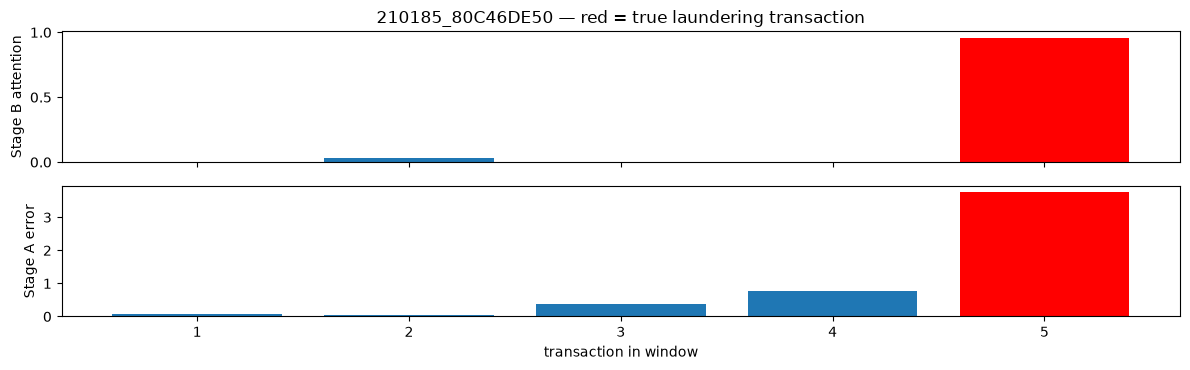
\includegraphics[width=0.85\textwidth]{figs/caso1.png}
\caption{Verdadero positivo 1. Atención del modelo final (arriba) y error de reconstrucción de la Etapa A (abajo) por transacción. En rojo, la transacción de lavado.}
\end{figure}

\textbf{Verdadero positivo 2 (fan-in).} Presenta el mismo patrón. La última transacción (USD 19,031) recibe 94\% de la atención, y su receptor ya había recibido dinero de 12 remitentes.

\begin{figure}[H]
\centering
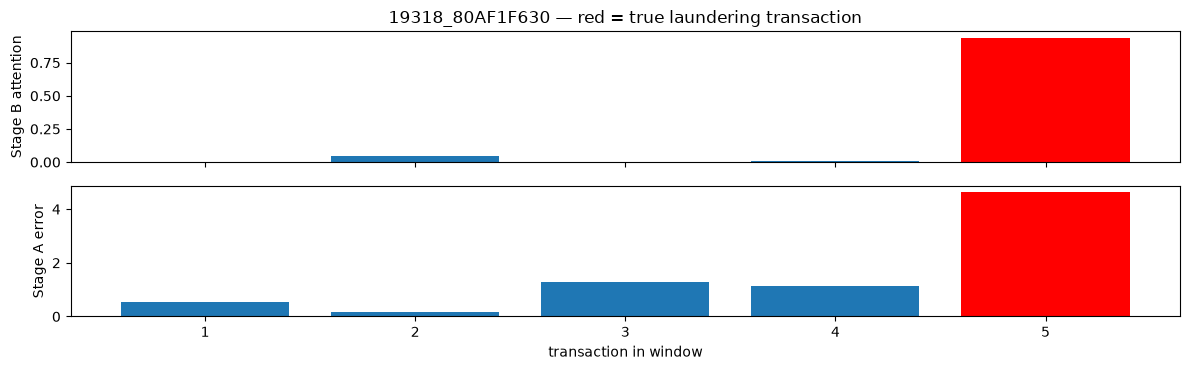
\includegraphics[width=0.85\textwidth]{figs/caso2.png}
\caption{Verdadero positivo 2.}
\end{figure}

\textbf{Verdadero positivo 3 (fan-in).} La ventana tiene 32 transacciones y solo la última es de lavado (USD 8,334 a un receptor nuevo). Recibe 98\% de la atención, aunque solo 22\% de la ventana usa ACH.

\begin{figure}[H]
\centering
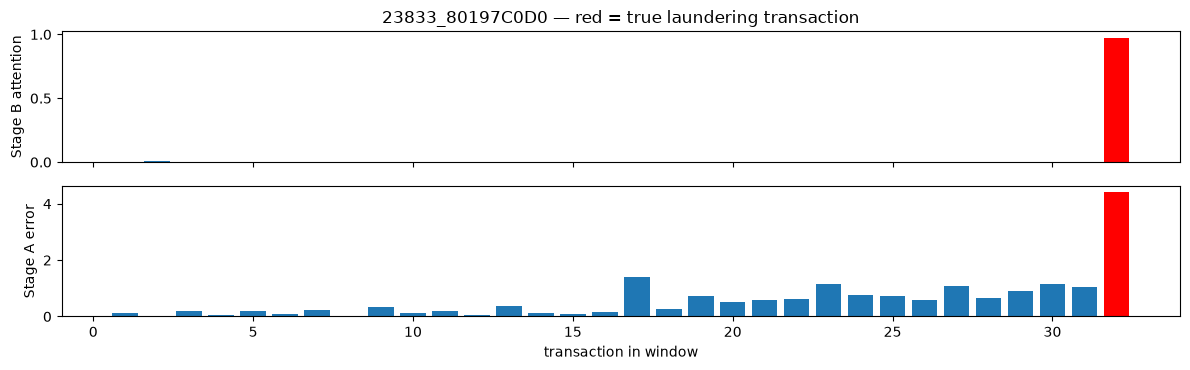
\includegraphics[width=0.85\textwidth]{figs/caso3.png}
\caption{Verdadero positivo 3.}
\end{figure}

\textbf{Falso positivo.} Un remitente legítimo hizo seis pagos por ACH. Dos fueron de exactamente USD 2,318 y sin separación en el tiempo, y uno fue de USD 0. Esto se parece a un fraccionamiento de montos, y el modelo no tiene forma de saber que el remitente es legítimo. La explicación permite al analista descartar la alerta.

\begin{figure}[H]
\centering
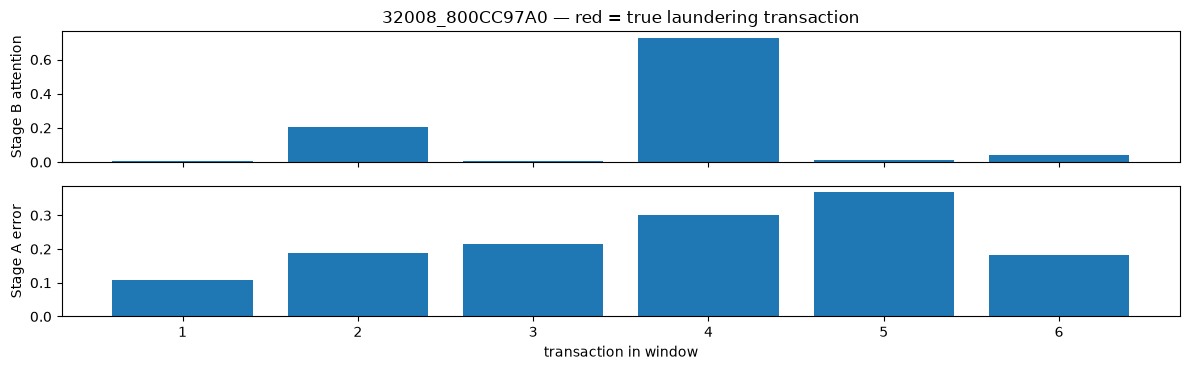
\includegraphics[width=0.85\textwidth]{figs/caso4.png}
\caption{Falso positivo.}
\end{figure}

\textbf{Falso negativo (bipartite).} La transacción de lavado es la número 2 de la ventana (USD 8,809 a un receptor nuevo), y la atención la encuentra con 58\%. Aun así, el clasificador ubicó al remitente en el percentil 82 de riesgo, es decir, más riesgoso que el 82\% de los remitentes y fuera del 5\% alertado. La Etapa A lo había ubicado en el percentil 99 de anomalía, pero con peso 1 esa señal no entra en la decisión final.

\begin{figure}[H]
\centering
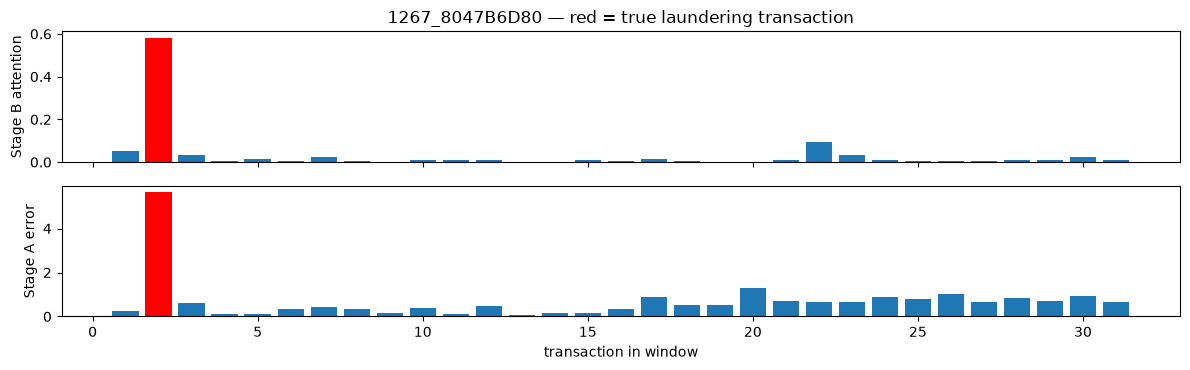
\includegraphics[width=0.85\textwidth]{figs/caso5.png}
\caption{Falso negativo.}
\end{figure}


\section{Limitaciones y camino a producción}
\label{sec:limites}

\textbf{Limitaciones.}
\begin{itemize}
  \item Los datos son sintéticos y tienen artefactos del simulador. Los resultados no se pueden extrapolar a remesas reales ni a su tasa de lavado.
  \item El modelo ve a cada remitente por separado, pero el lavado es un fenómeno de red. Detecta la mayoría de los patrones conocidos, pero no el lavado sin tipología. Los remitentes con una sola transacción (31\%) quedan fuera del alcance.
  \item El preentrenamiento no mejoró el resultado de forma consistente. Habría que probar otro objetivo de preentrenamiento.
  \item Cada modelo se entrenó una sola vez, y los resultados cambian un poco entre corridas. Por eso no se puede separar un efecto real del ruido.
\end{itemize}

\textbf{Para llevarlo a producción en una remesadora.}
\begin{itemize}
  \item \textbf{Datos reales etiquetados.} Por ejemplo, los reportes de operaciones sospechosas.
  \item \textbf{Calibración y umbrales.} Las probabilidades del modelo no están calibradas, porque el entrenamiento usó pocos negativos. Calibrar significa ajustarlas a la frecuencia real de lavado. El umbral debe fijarse con la capacidad real de revisión y con el reglamento del Decreto 15-2026.
  \item \textbf{Monitoreo y reentrenamiento.} Se debe vigilar el volumen de alertas, los cambios en los datos y la proporción de alertas reales, y reentrenar de forma periódica.
  \item \textbf{Revisión humana y gobierno del modelo.} Cada alerta pasa por un analista con la explicación a la vista, y queda registrada para auditoría.
\end{itemize}

\section{Uso de IA generativa}

Se usó Claude (Anthropic), a través de Claude Code, para reorganizar el código de las etapas A y B, documentar el notebook, verificar las referencias y la ley vigente, construir el demo web y redactar el borrador de este reporte. Las decisiones de diseño fueron propias. Se decidió usar un autoencoder encoder-decoder en la Etapa A, agregar un MLP como línea base y comparar LSTM y Transformer en ambas etapas. También se fijó el umbral en el 5\% de remitentes alertados, y se cuestionó el umbral de mejor F1 que se había implementado. El detalle completo, con la verificación y los errores de la IA, está en el archivo \texttt{AI.md}.

\printbibliography

\end{document}
